\begin{figure}
\centering
  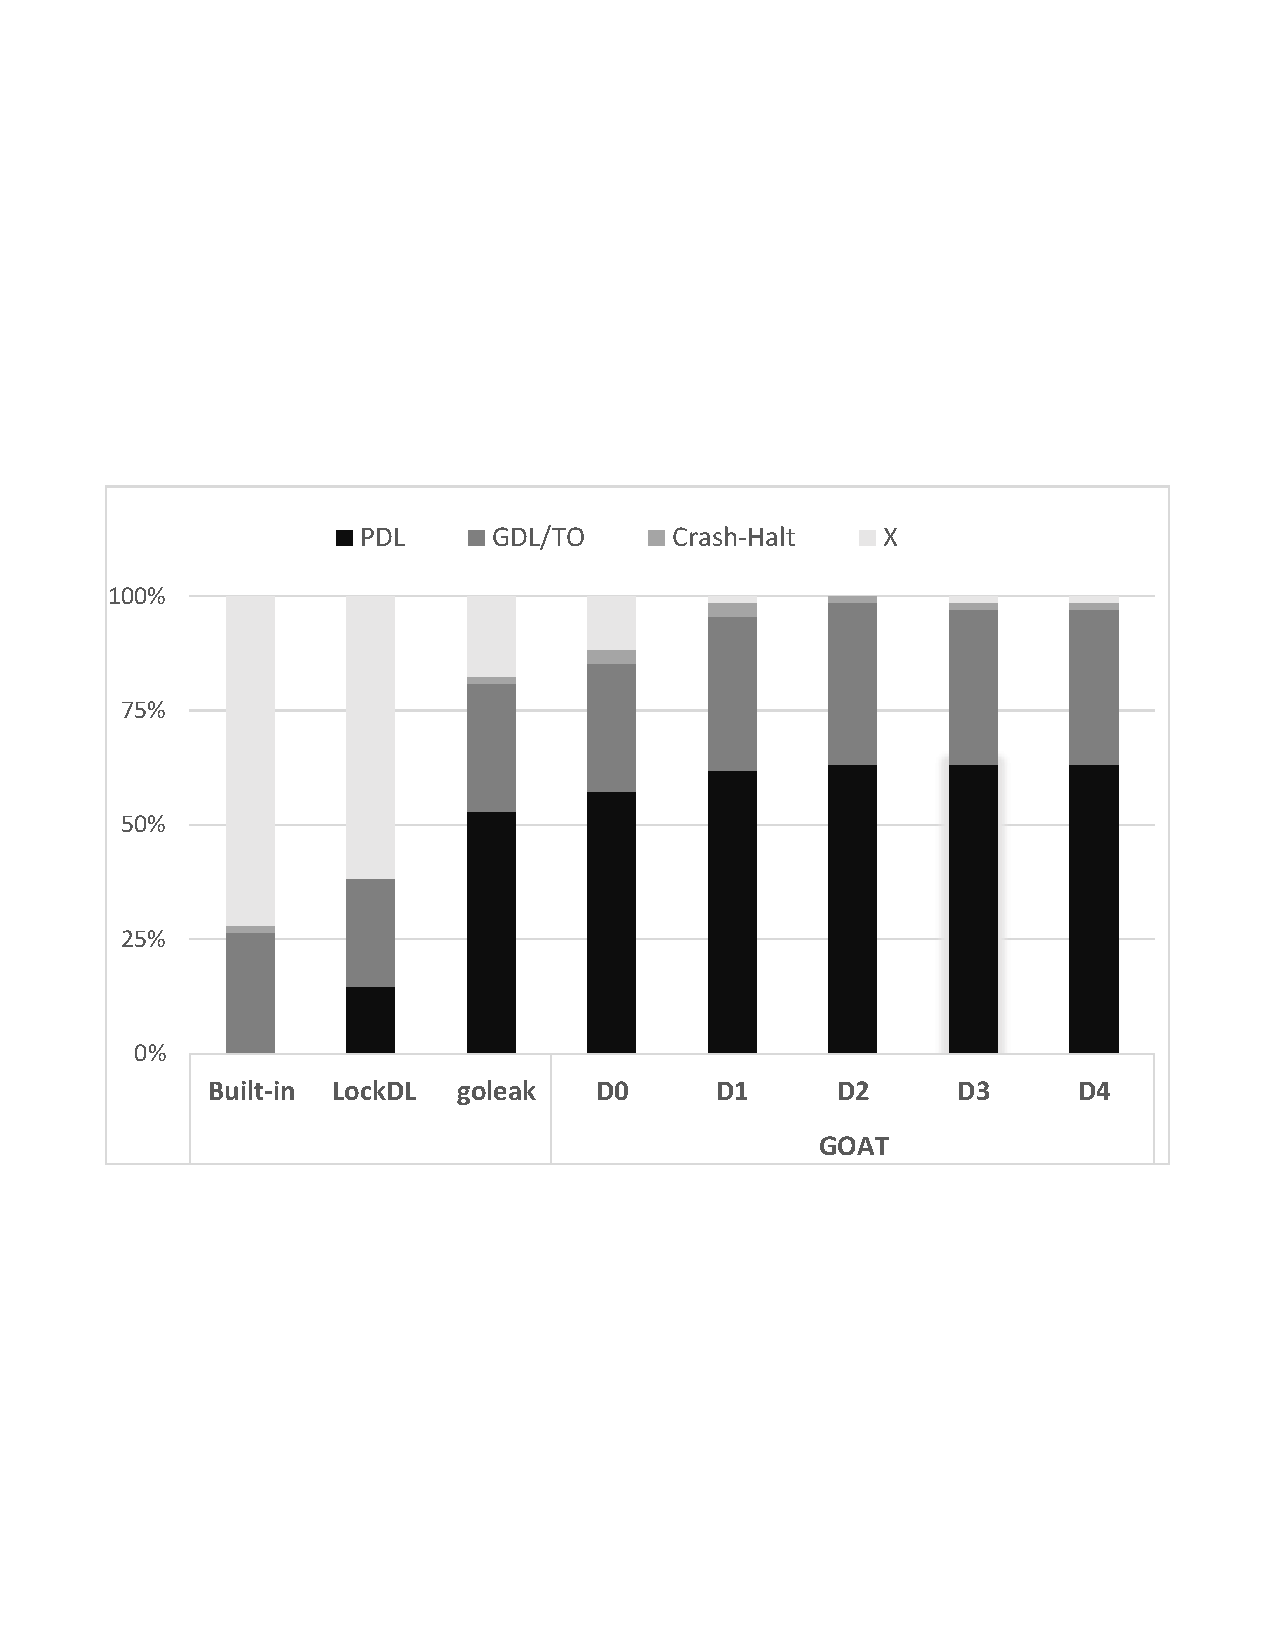
\includegraphics[width=.95\linewidth]{figs/P4_detections.pdf}
  \caption{Histogram of detected bugs by each tool performed on 68 GoKer blocking bugs. PDL: partial deadlock, GDL/TO: global deadlock, Crash/Halt: causes the program to crash or halt during detection.}
  \label{fig:detection}
\end{figure}


\begin{figure}
\centering
  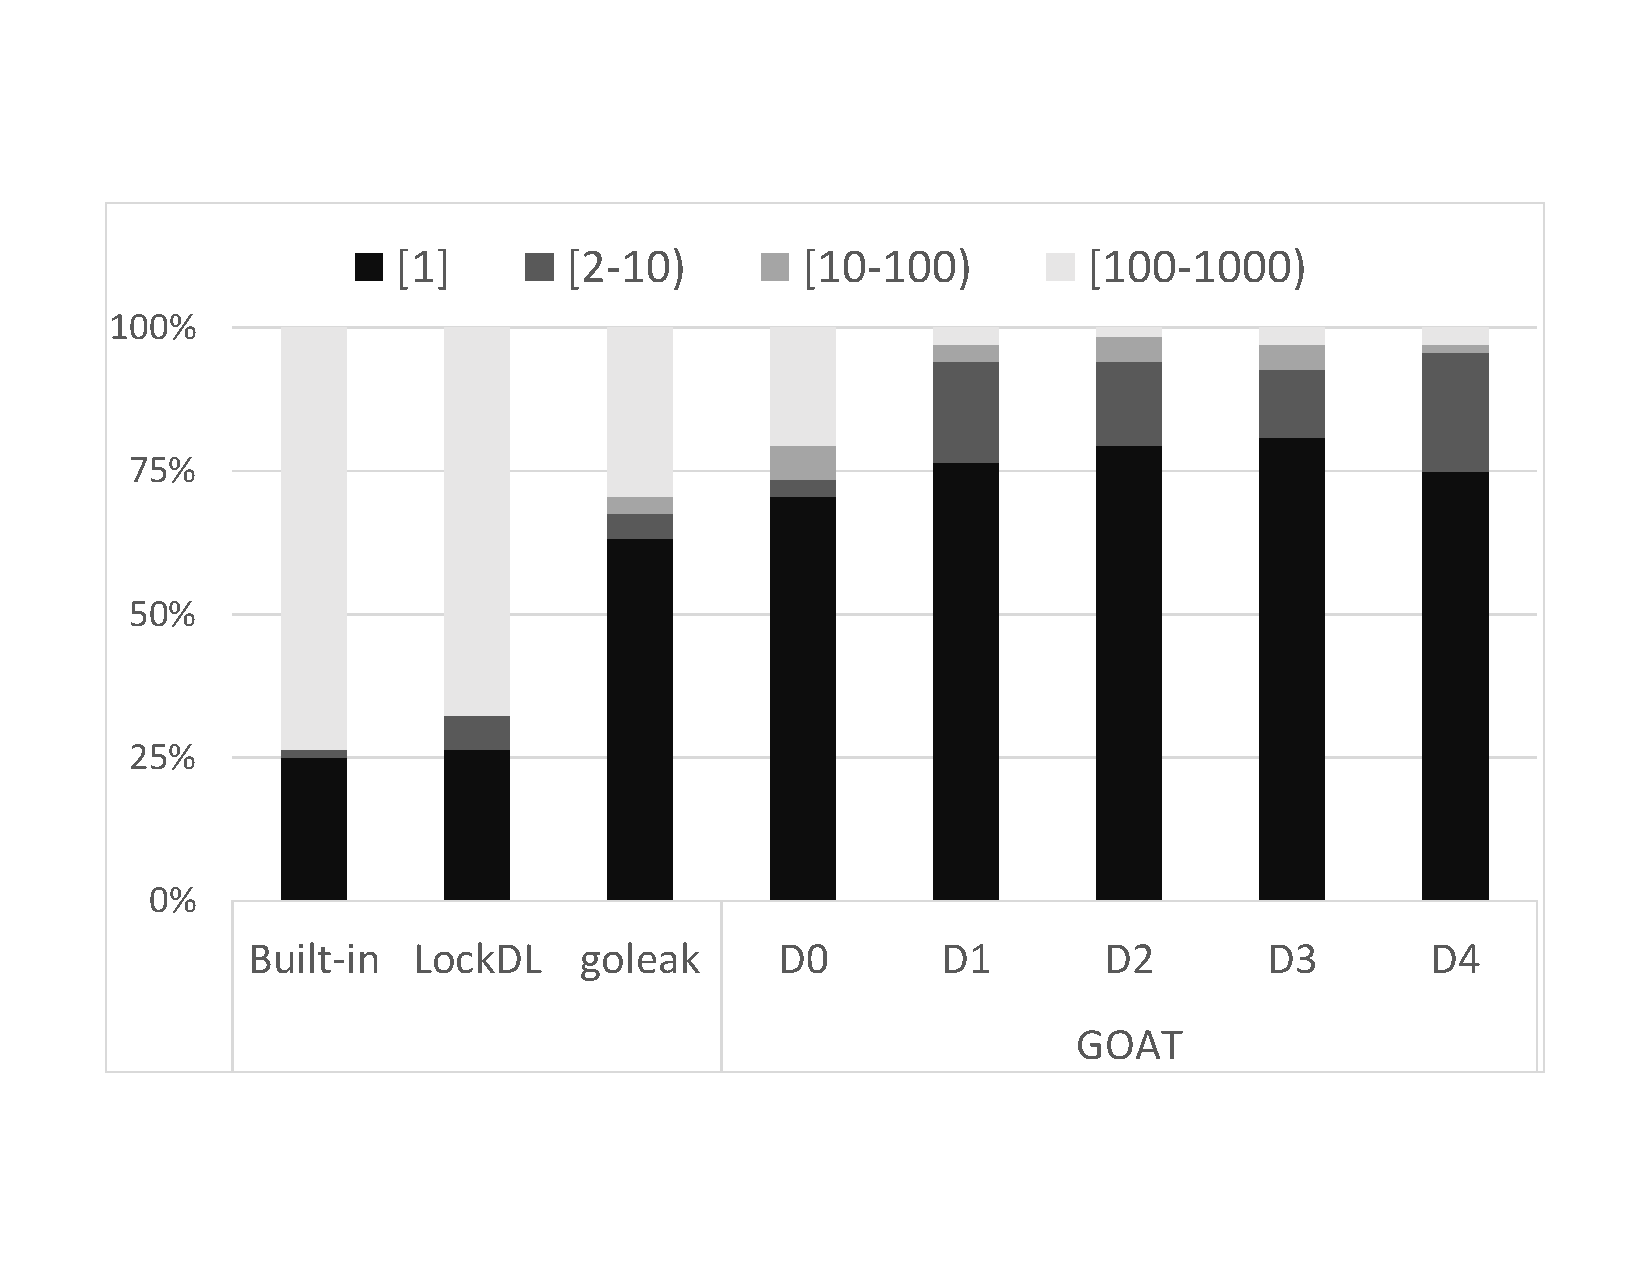
\includegraphics[width=.95\linewidth]{figs/P4_runs2.pdf}
  \caption{Percentage distribution for the average required number of iterations (falling into each of the four given intervals) by each tool to detect 68 GoKer blocking bugs.}
  \label{fig:runs}
\end{figure}


%
% \begin{figure*}
% \begin{minipage}{.49\textwidth}
% \centering
%   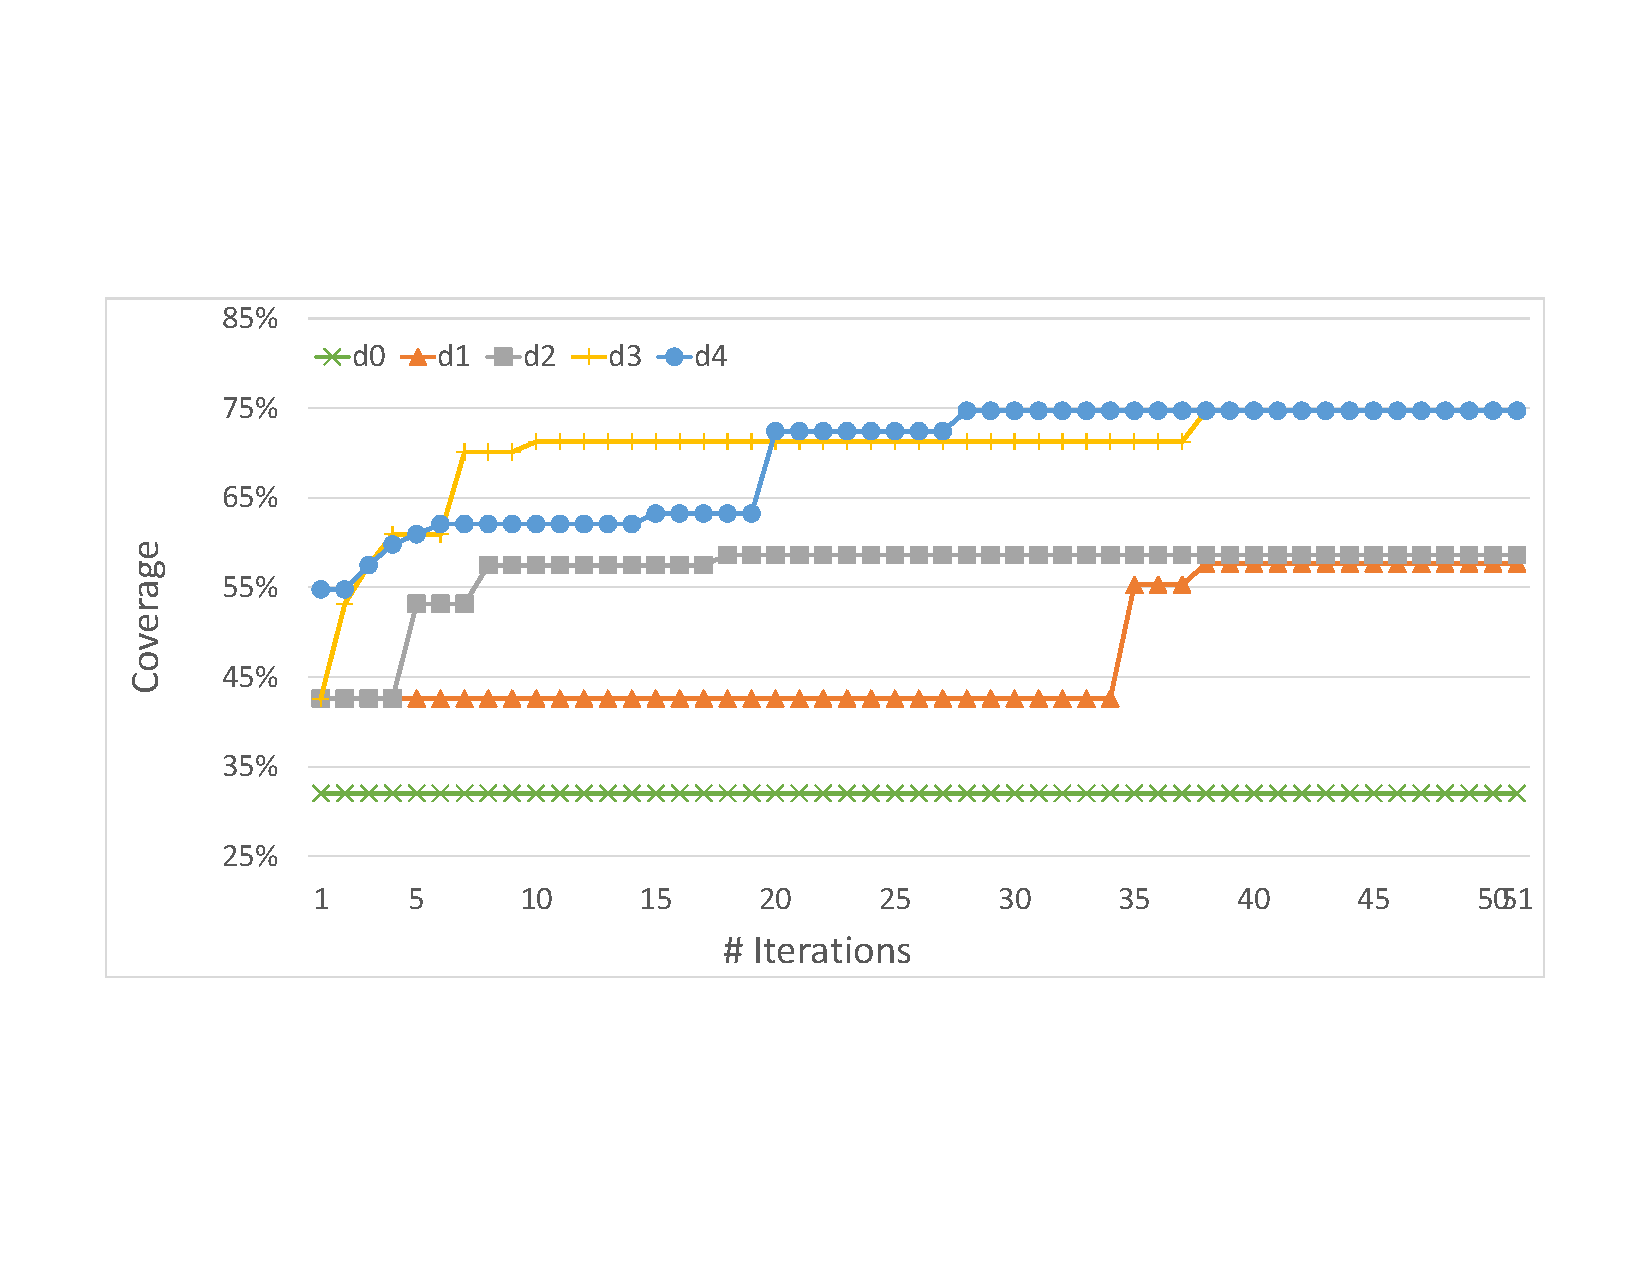
\includegraphics[width=.95\linewidth]{figs/coverage_etcd7443.pdf}
%   \caption{etcd7442 coverage}
%   \label{fig:etcd_coverage}
% \end{minipage}
% \begin{minipage}{.49\textwidth}
% \centering
%   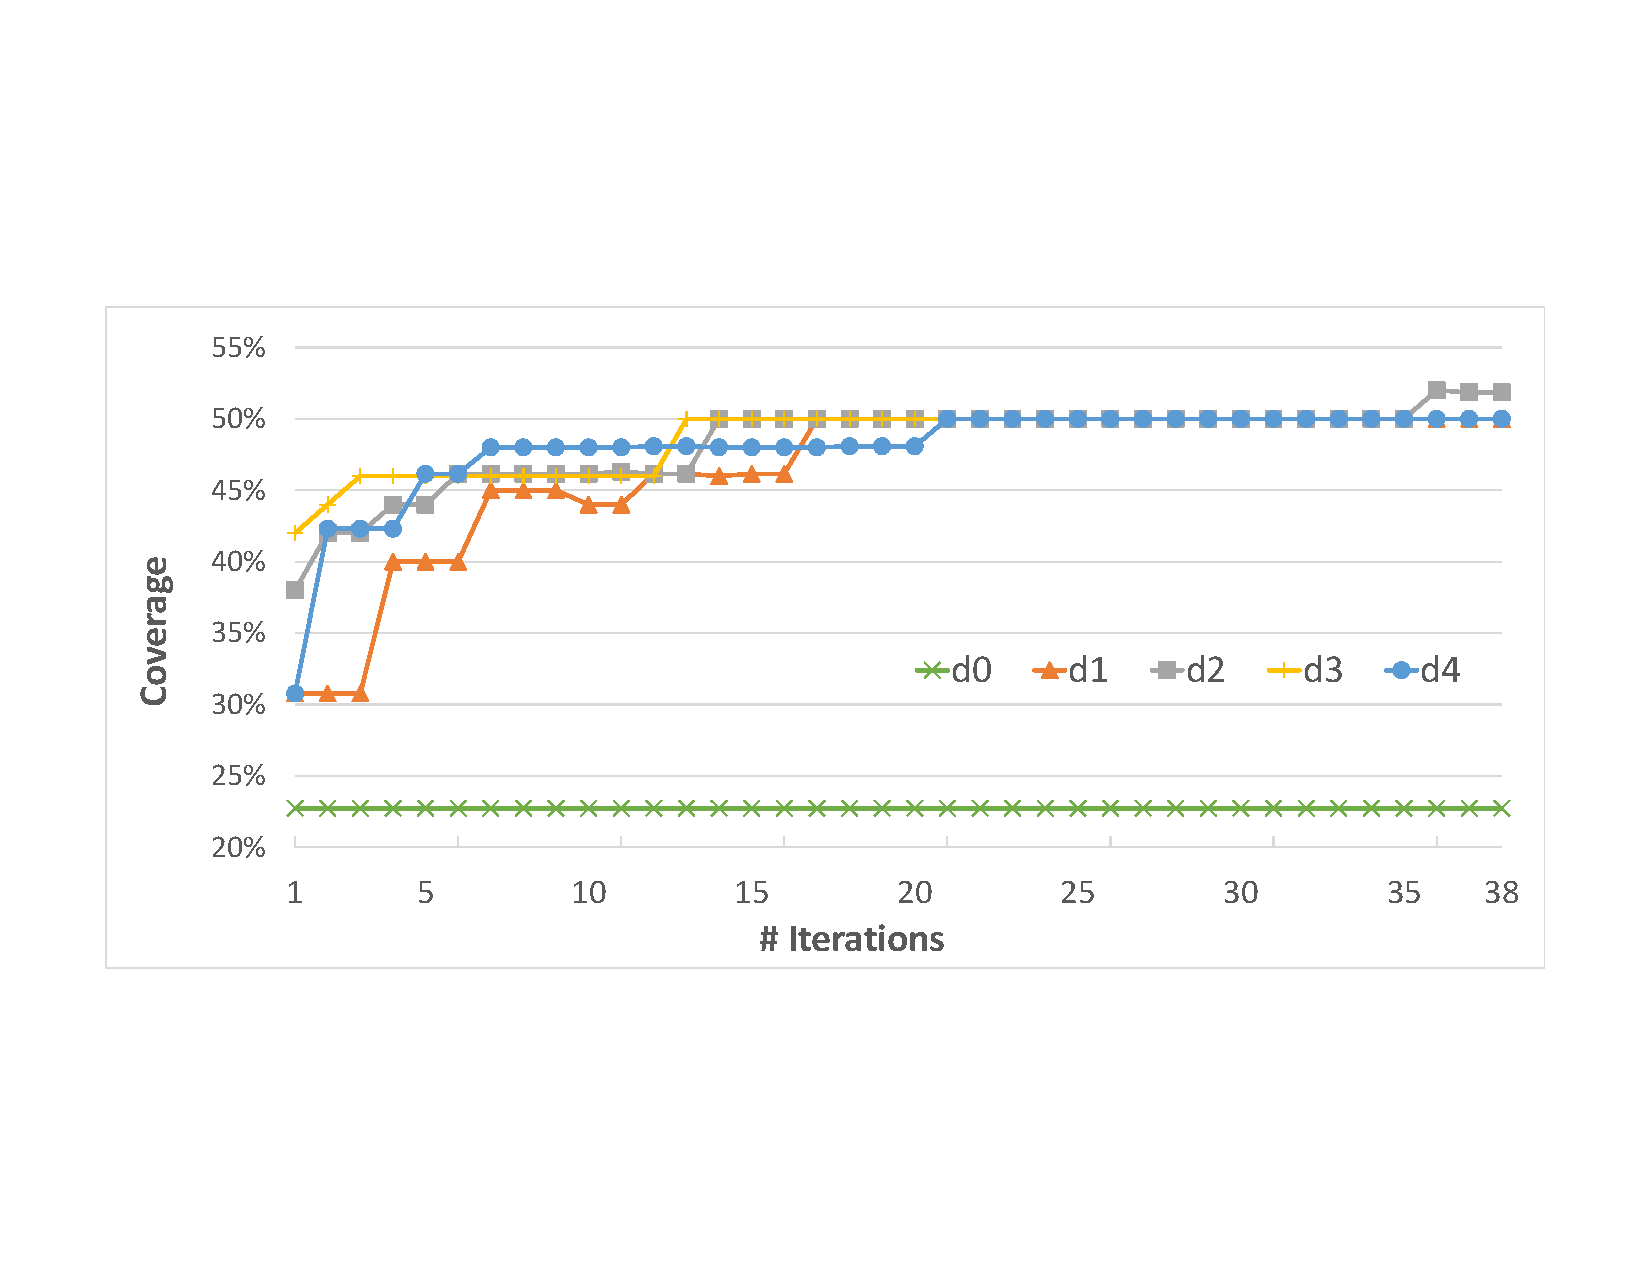
\includegraphics[width=.95\linewidth]{figs/coverage_kubernetes11298.pdf}
%   \caption{kuberenetes11298 coverage}
%   \label{fig:kubernetes_coverage}
% \end{minipage}
% \end{figure*}

\subsection{Deadlock Detection}
\label{sec:dl_evaluation}
We assess the ability of \goat and its variations in detecting bugs with the minimum number of executions required to expose the bug.
%
We have compared \goat against three existing dynamic detectors:
\begin{itemize}
  \item \textit{Built-in} deadlock detector: It is an embedded mechanism in the standard Go runtime. The mechanism periodically makes sure that the queue of \textit{runnable} goroutines is never empty until the main goroutine terminates. If the queue is empty and the main goroutine has not terminated yet (\ie, main is blocked), it throws a runtime error.
  \item \textit{LockDL} \cite{lockdl}: This tool intercepts with all mutex locks and unlocks of the target application to maintain a ``lock-set'' data structure. \textit{LockDL} issues warning during runtime when it finds a circular wait in the lock-set or double-locking the same lock. It has a timeout mechanism for the application that traps into global deadlocks (30 seconds).
  \item \textit{goleak} \cite{goleak}: This leak detector from Uber checks the program stack at the end of the main goroutine's execution to find the application-level goroutines that remained in the stack (\ie, leaked).
\end{itemize}


\begin{figure*}
     \centering
     \begin{subfigure}[b]{0.46\textwidth}
        \centering
        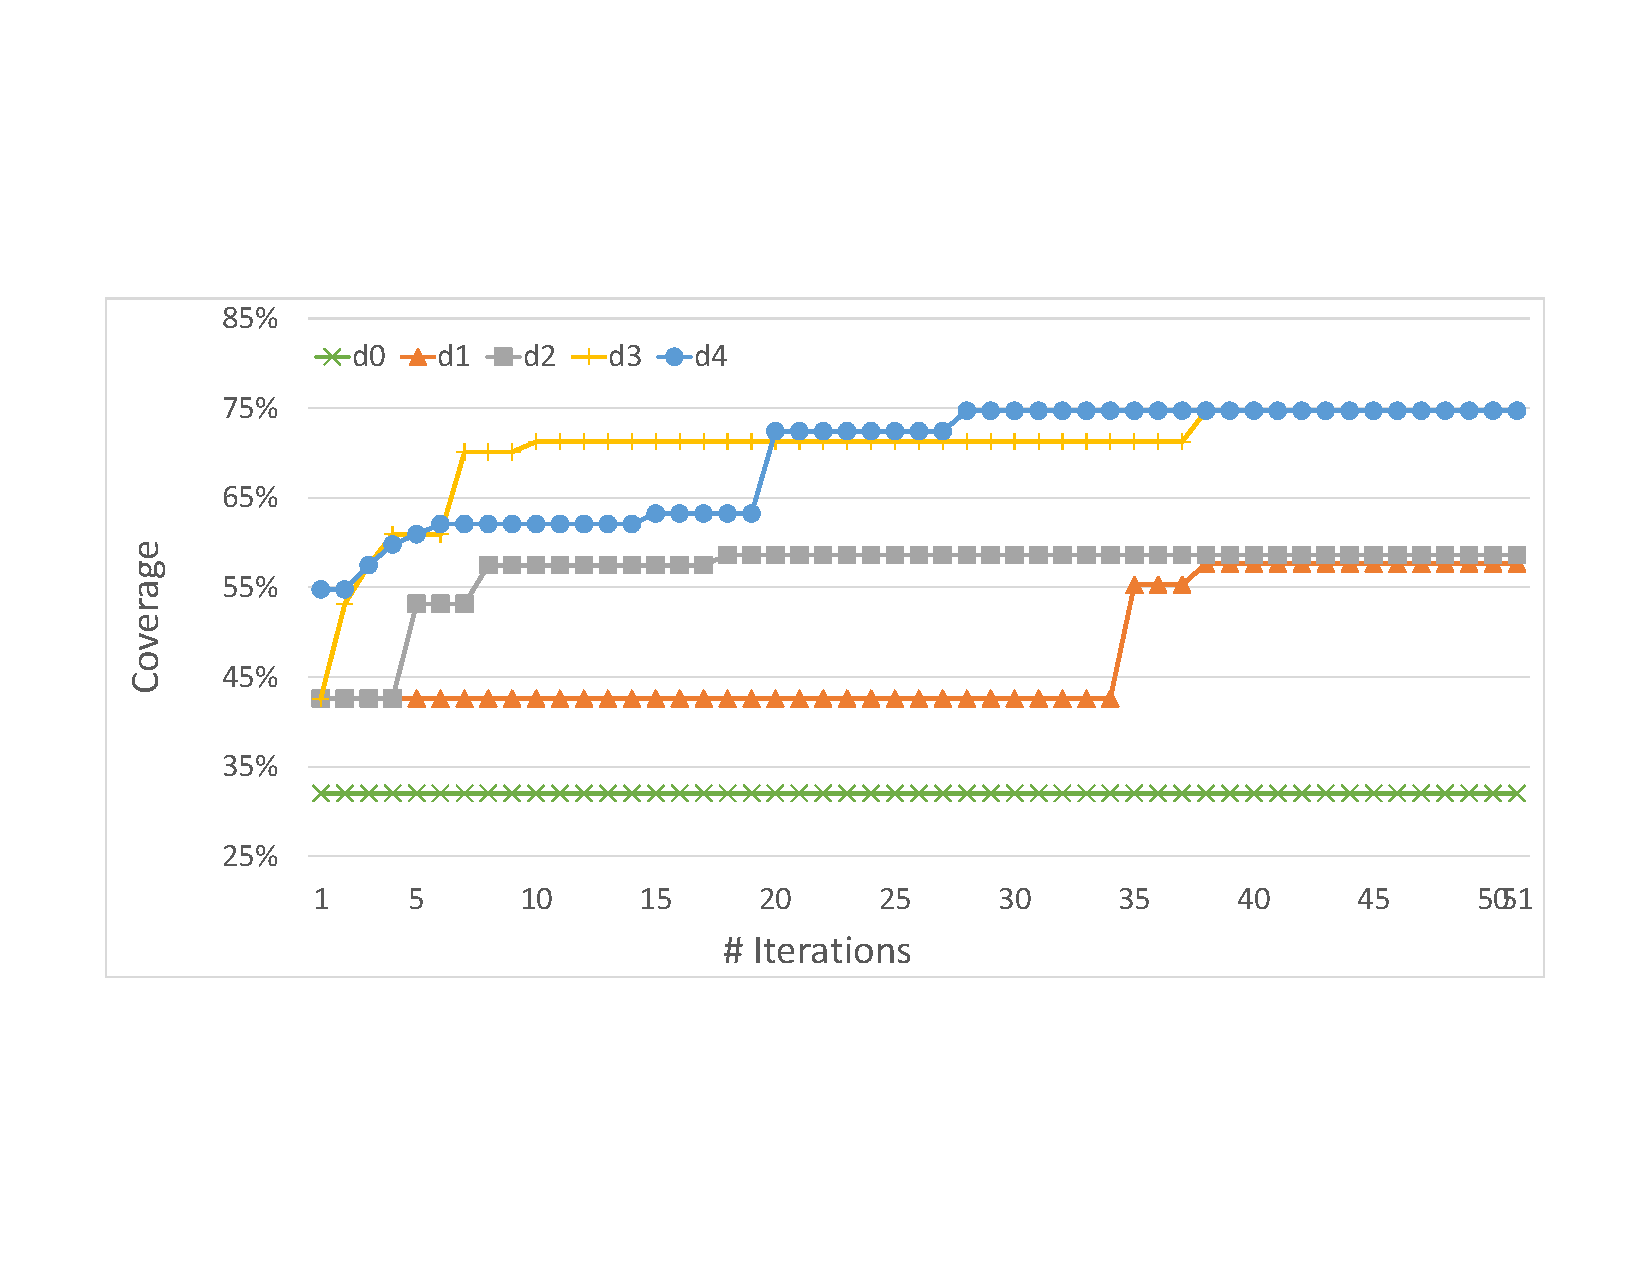
\includegraphics[width=\textwidth]{figs/coverage_etcd7443.pdf}
        \caption{\texttt{etcd7443}}
        \label{fig:etcd_coverage}
     \end{subfigure}
     \hfill
     \begin{subfigure}[b]{0.46\textwidth}
       \centering
       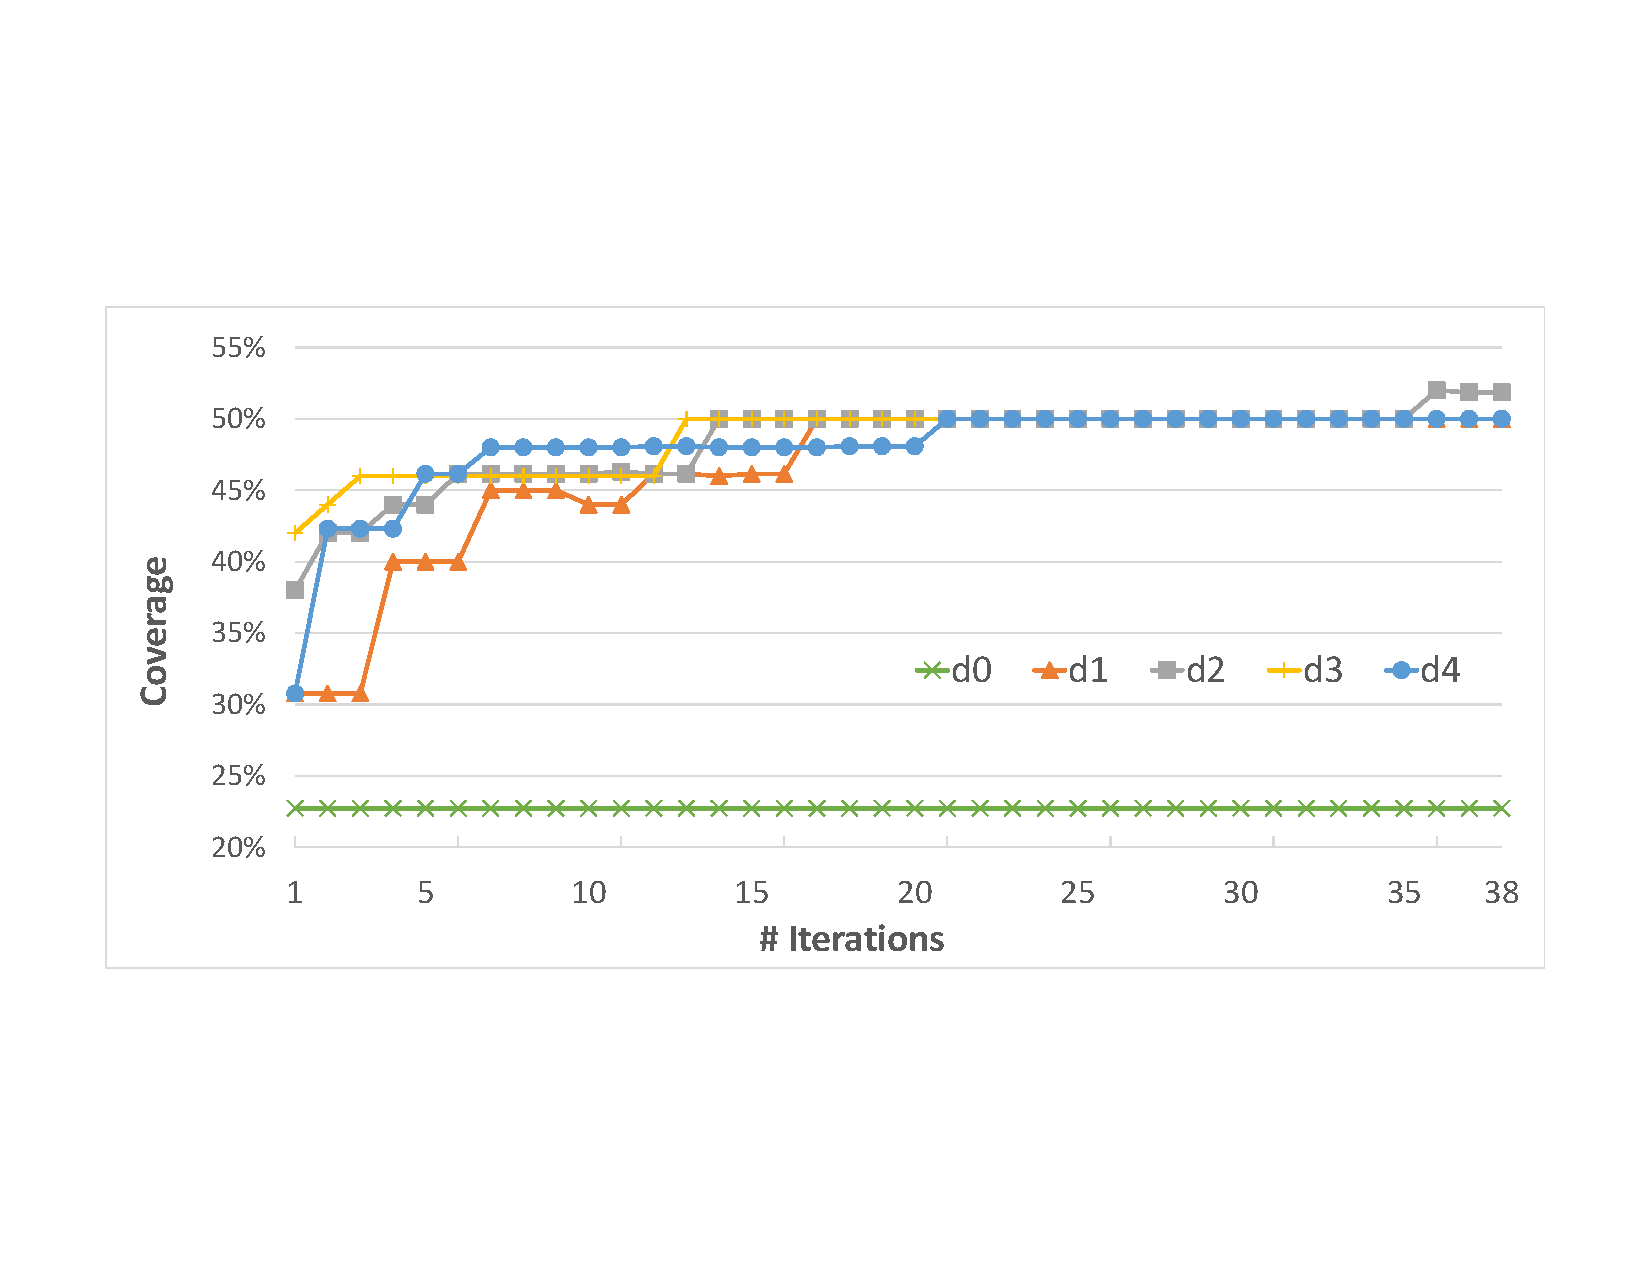
\includegraphics[width=\textwidth]{figs/coverage_kubernetes11298.pdf}
       \caption{\texttt{kuberenetes11298}}
       \label{fig:kubernetes_coverage}
     \end{subfigure}
        \caption{Coverage percentage after each iteration of \goat with various $D$ values for two representative bugs~\cite{yuan-gobench-cgo21}. Iterations on the Y axis of figures end when the respective bug is first detected. For example, \goat($D2$) detects the bug in \texttt{kuberenetes11298} after 38 executions at 52.23\% coverage percentage.}
        \label{fig:coverage}
\end{figure*}



All experiments are performed on a server with Intel(R) Xeon(R) CPU E7 processor (64 total cores with two threads per core and eight cores per socket), 512 GB of RAM with Ubuntu 5.4.0 and Go version 1.15.6.
%
Table \ref{tab:comparison} shows the details of results obtained from 1000 executions of each tool per bug.
%

%


%
Figure \ref{fig:detection} and table \ref{tab:comparison} show that variations of \goat outperforms other detector by discovering the bug in 100\% of the GoKer blocking benchmark.
%
Figure \ref{fig:runs} and highlighted cells of table \ref{tab:comparison} show that the idea of injecting random delays around concurrency usage points in the program drastically reduces the required number of testing iterations until the bug occurs.
%
$D0$ means \goat did not delay the program at any point and $D4$ means that the target program has been delayed up to four times around its CU points.
%
Figures \ref{fig:detection} and \ref{fig:runs} also state that the increase in the delay bound of \goat does not necessarily increase the chance of exposing the bug.
%
For example, the row of bug \texttt{serving\_2137} in table \ref{tab:comparison} show that only \goat $D2$ were able to detect the bug.




\subsection{Coverage Analyis}
We picked two representative bug kernels \texttt{etcd7443} and \texttt{kubernetes11298} to evaluate the coverage idea on them as they both have extensive use of channels, mutexes, conditional variables, nested selects within nested for loops, and the buggy interleaving is proved to be rare to happen.
%
figures \ref{fig:etcd_coverage} and \ref{fig:kubernetes_coverage} show the gradual increase in coverage percentage during testing iterations for different values of $D$.
%
Recall that $D$ is the bound on the number of yields that we inject to the native execution of a given program to perturb the scheduler around concurrency usages.
%
With the increase of $D$, the coverage percentage increase rate also grows.
%
With lower values of $D$, the coverage percentages start at lower values and increase more slowly over iterations.
%
The reason is that the scheduler does not get to explore different interleavings (thus different coverage scenarios), and over iterations, the program executes more deterministic regarding coverage requirements.
%
However, higher $D$ does not necessarily increase the coverage ($D2$ and $D4$ in figure \ref{fig:kubernetes_coverage}).
%
The gradual increase of the coverage percentage and non-uniform increase rates for different values of $D$ reflects the effectiveness of our proposed coverage metric.
%
The drop in coverage for $D1$ in figure \ref{fig:kubernetes_coverage} is because of the new coverage requirements (\eg, a new goroutine is spawned and executing some concurrency primitives) that were encountered during testing execution.
%
